\section{Gestión de riesgos}
El motivo de esta sección viene de la definición del modelo en espiral como metodología clave para el desarrollo de este proyecto. Este modelo recoge la identificación y gestión de riesgos como pieza fundamental del ciclo de vida, y en un proyecto con tal complejidad técnica y con tantos dispositivos involucrados, es indispensable tener un plan de acción ante cualquier incidente.
\\ \\
Con tantos dispositivos que gestionar, el proceso de configuración de estos puede llegar a ser algo pesado, y más si alguno de estos falla o se rompe. Si se rompiese o se corrompiese una tarjeta SD de una Raspberry Pi habría que reinstalar y configurar todos los paquetes a mano, proceso que puede ser bastante largo puesto que requiere de interacción humana. Para evitar esto se ha tomado la dedcisión de crear un script de aprovisionamiento tanto para la Nvidia Jetson Nano como para las Raspberry Pis, de esta manera, en caso de que una tarjeta SD se averiase, bastaría con cambiarla, configurar el protocolo SSH para acceder remotamente a ella y ejecutar el script. Cuando el proceso terminase el dispositivo estaría listo para poder ejecutar el proyecto sin ningún problema.
\\ \\
Las tareas de inteligencia Artificial no son especialmente livianas para un dispositivo, lo que durante un entrenamiento prolongado en el tiempo podría incurrir en un aumento de temperatura de este. Para evitar que los dispositivos alcancen temperaturas elevadas o que sufran cualquier tipo de cortocircuito por su manipulación inadecuada se ha optado por instalarlos en un rack (Fig \ref{fig:RackRaspberry}). Esta carcasa aparte de proteger los dispositivos viene equipada con ventiladores que ayudaran a que la temperatura de estos sea siempre la adecuada.

\begin{figure}[thbp]
    \centering
    \fbox{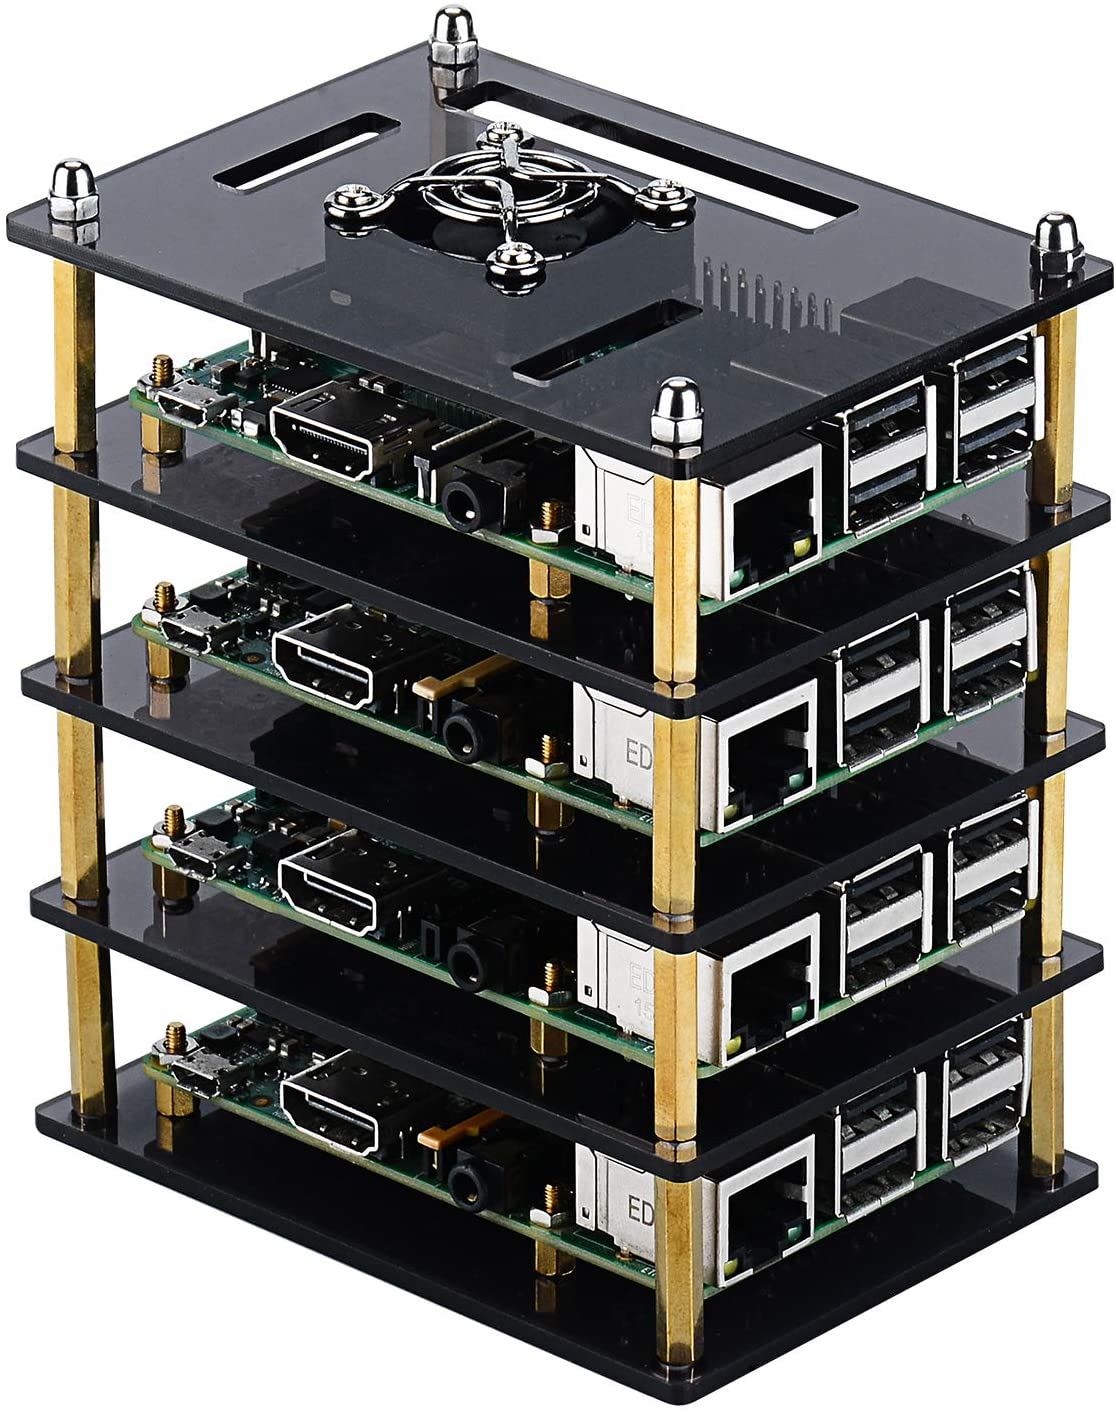
\includegraphics[width=0.3\textwidth]{Figuras/RaspBerryRack.jpg}}
    \caption{Rack para Raspberry Pi (Fuente: Amazon\autocite{ParaRaspberryPi})}
    \label{fig:RackRaspberry}
\end{figure}

Durante el desarrollo se tiene que acceder a estos dispositivos en multitud de ocasiones, para ello se utiliza el protocolo SSH. Sin embargo, al realizarse este proyecto en un ámbito doméstico, existe la probabilidad de que el router sea reiniciado o apagado por cualquier causa externa al proyecto. En tal caso puede que las direcciones IP sean sustituidas y haya que realizar un análisis de la red o acceder fisicamente a estos dispositivos para averiguar la IP. Para evitar este proceso se ha instalado el paquete \textit{AVAHI}\footnote{AVAHI es un servicio que facilita el descubrimiento de dispositivos en la red local a través de mDNS/DNS-SD.} que permite acceder mediante SSH a las raspberrys sustituyendo la dirección IP por el nombre de servidor de los dispositivos.
\\ \\
Para gestionar los cambios que se irán haciendo sobre el software sin problemas es indispensable contar con herramientas de control de versiones. Estas herramientas permiten gestionar cuándo se han realizado qué cambios y en caso de necesitarse se podrían revertir con facilidad. En este caso, tanto para el desarrollo del proyecto como para el desarrollo de la memoria se utilizará Git como controlador de versiones. Además, se utilizará Github como repositorio de código en la nube, para así poder clonar el repositorio a los dispositivos facilmente.
